% Figure from MATH 591 notes, section 3. Compile with the notes preamble.
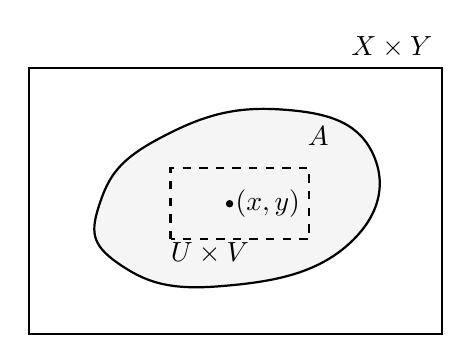
\begin{tikzpicture}[scale=0.75]
    \draw[thick] (0,0) rectangle (7,4.5);
    \node[anchor=south east] at (7,4.5) {$X \times Y$};
    \draw[thick, fill=gray!8] plot [smooth cycle, tension=0.8] coordinates {(1.5,1.2) (3.2,0.8) (5.4,1.5) (5.8,3.1) (4.2,3.8) (2.2,3.3) (1.2,2.2)};
    \node at (4.9,3.35) {$A$};
    \filldraw (3.4,2.2) circle (1.5pt) node[anchor=west, inner sep=2pt] {$(x,y)$};
    \draw[dashed, thick] (2.4,1.6) rectangle (4.75,2.8);
    \node[anchor=north west, inner sep=1pt] at (2.35,1.6) {$U \times V$};
\end{tikzpicture}
